\chapter{SDN Control Plane Scalability} \label{sec:sdn_scalability} 

This dissertation contends that control plane applications can scale aspects of
computer network functionality. In our exploration we extensively employ the SDN
design paradigm and the \of abstraction, primarily due to two core
functional properties.  Firstly, the clean separation of the network control
and data plane is inherently backwards-compatible with existing network
applications and interoperable with existing network devices.  The evolution of
the control plane of a network does not affect data plane protocol support and
allows progressive deployment in production networks.  Secondly, the \of control
abstraction is sufficiently generic to support various control approaches. The
protocol supports reactive and proactive control schemes, while the flow
definition granularity can be dynamically controlled to match the environment
requirements. The following chapters of this thesis employs \of to
address two diverse network scalability problems. 

This chapter presents an extensive scalability analysis of available SDN
technologies. Our exploration provides an in-depth analysis of the limitations
of existing implementation efforts and their impact on data plane performance.
The work focuses on implementations of version 1.0 of the \of protocol, the
predominant production-level protocol instantiation of SDN.  We present two
measurement platforms: \oflops and \sdnsim.  \oflops is a high precision \of
switch micro-benchmark platform. Using \oflops, we implement a set of benchmark
tests and characterise the performance of elementary protocol interactions.
\sdnsim is a macro-benchmark \of platform, which extends the Mirage
framework~\mycite{madhavapeddy2013} to support large scale \of-based network
simulations and emulations.  Using \sdnsim, experimenters can import
\oflops switch profiles into their experiment and test the performance of their
SDN design.

In this Chapter, we present the motivations (Section~\ref{sec:oflops-intro})
and the design overview of \oflops (Section~\ref{sec:oflops-design}). We select
a number of off-the-self \of switches (Section~\ref{sec:oflops-switches}) and
assess the elementary protocol interaction performance
(Section~\ref{sec:oflops-result}). Furthermore, we discuss some of limitations
in network experimentation and present \sdnsim (Section~\ref{sec:sdnsim-intro})
and its architecture (Section~\ref{sec:experimentation}). Finally, we assess
the performance scalability and fidelity of \sdnsim
(Section~\ref{sec:sdnsim-precision}), along with a measurement study of control
scalability over the fat-tree topology (Section~\ref{sec:rdsf-eval}), and
conclude our work (Section~\ref{sec:modeling:summary}). 

\section{Network Control Micro-benchmark} \label{sec:oflops-intro}

Despite the recent introduction of the SDN paradigm, the research community has
already proposed many novel control architectures, presented
extensively in Section~\ref{sec:background:ofapp}. These architectures address
significant problems of modern networking, but their deployment in production
environments is not straightforward.  Computer networks have become a vital asset
for modern enterprises.  High availability and performance are critical and any
control plane modification must fulfil these criteria, requiring extensive
testing and performance characterisation.  \mycitet{Weissmann:va} present the
deployment experience of the first \of network in the Computer
Science department of Stanford University, and report significant performance and
reliability problems.  The performance limitations were significantly
influenced by the inability of the hardware switching platform to process \of
interactions at high rates.  Fundamentally, the SDN development toolchain lacked
generic tools to assess \of scalability.  Traditional switch performance models
use metrics like packet latencies and MAC table size. The control decoupling of
the SDN paradigm expands the interaction freedom between a controller and a
switch device, and effectively increases the complexity of characterising switch
performance. 

In order to fulfil the requirement for \of switch performance evaluation, we
developed \oflops\footnote{\oflops is under the GPL licence and can be
  downloaded from \url{http://www.openflow.org/wk/index.php/Oflops}}, a
measurement framework enabling rapid development of performance tests for
hardware and software \of switch implementations. To better understand the
behaviour of the tested \of implementations, \oflops combines
\of control and data plane measurements. To ensure
sub-millisecond-level accuracy of the measurements, we bundled the \oflops
software with specialized hardware in the form of the NetFPGA
platform\footnote{\url{http://www.netfpga.org}}.  Note that if the tests do not
require millisecond-level accuracy, commodity hardware can be used instead of
the NetFPGA \mycite{pam-accuracy}.

\section{\oflops Design}\label{sec:oflops-design}

\begin{figure}
\centering
\subfigure[NetFPGA packet]{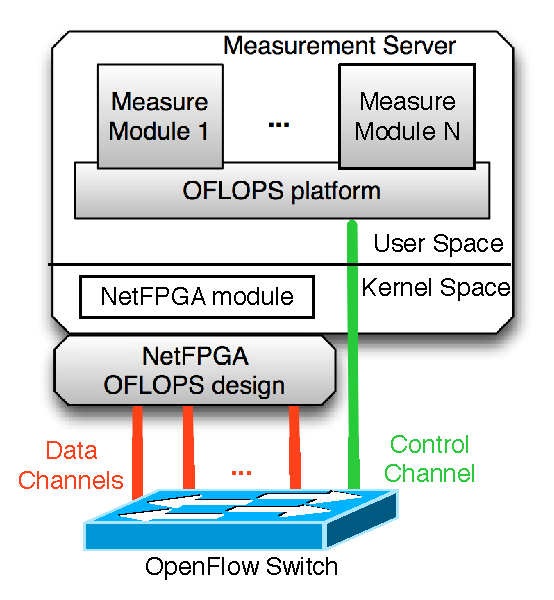
\includegraphics[width=0.30\textwidth]{Chapter1/Chapter1Figs/oflops-design-netfpga}\label{fig:oflops_design_netfpga}}
\subfigure[Kernel-space]{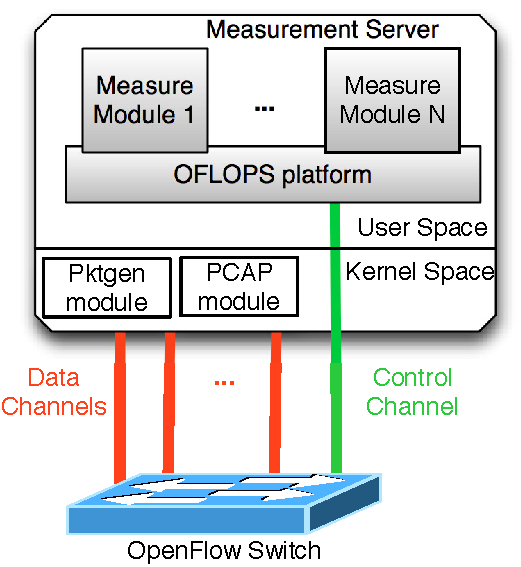
\includegraphics[width=0.30\textwidth]{Chapter1/Chapter1Figs/oflops-design-kernel}\label{fig:oflops_design_kernel}}
\subfigure[User-space]{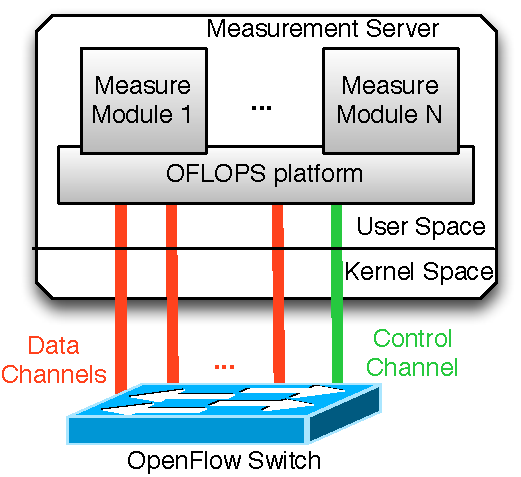
\includegraphics[width=0.30\textwidth]{Chapter1/Chapter1Figs/oflops-design-userspace}\label{fig:oflops_design_userspace}}
\label{fig:oflops_design}
\caption[\oflops architecture]{\oflops enables the development of
  custom multi-channel measurement experiments and supports: 1) the high accuracy
  NetFPGA packet generator hardware design
  (Figure~\ref{fig:oflops_design_netfpga}), 2) the kernel space {\tt pktgen}
  traffic generation module and the PCAP packet capturing
  module~(Figure~\ref{fig:oflops_design_kernel}), 3) a userspace packet capture
  and generation library (Figure~\ref{fig:oflops_design_userspace}).}
\end{figure}

Measuring \of switch implementations is a challenging task in terms of
the characterization of accuracy, noise suppression and precision.  Performance
characterization is non-trivial, as most \of-enabled devices provide rich
functionality but do not disclose implementation details. In order to understand
the performance impact of an experiment, multiple input measurement channels
must be monitored concurrently, such as data and control channels. Furthermore,
current controller frameworks, like~\mycitet{gude08,floodlight}, are designed for
production networks and incur significant measurement noise. Such controllers
employ asynchronous processing libraries and multi-thread execution models, to
maximize the aggregate control channel processing throughput, and provide
high-level programming interfaces that require multiple data structure
allocation and modification during packet processing.  The processing time for a
specific \of message, especially at high rates, is subject to multiple aspects,
like thread scheduling policy and asynchronous library execution
logic~\mycite{Jarschel2012}.  Measurement noise suppression in the control plane
is required from the controller framework to minimize message processing and
delegate processing control to the measurement module.  Finally, sub-millisecond
precision in software is subject to unobserved parameters, like OS scheduling
and clock drift. The result of these challenges is that meaningful, controlled,
repeatable performance tests are non-trivial in an \of environment.

\oflops has a low overhead abstraction, enabling interaction with an
\of-enabled device over multiple data channels.  The platform provides a
programming API, allowing control of multiple information sources: data and
control channels, and SNMP\@, following an event-driven architecture.
Interactions over each channel are transformed into semantically meaningful
events and the experimenter can register callbacks to handle them programatically.
\oflops is implemented in C, and experiments are compiled as shared libraries,
loaded at run-time using a simple configuration interface.  A schematic of the
platform is presented in Figure~\ref{fig:oflops_design}, while
\mycitet{oflops-manual}~provides further details regarding the \oflops
programming model.

The platform is implemented as a multi-threaded application and takes
advantage of modern multicore environments. To reduce latency, our design
avoids concurrent access controls: we leave any concurrency-control complexity 
to individual module implementations. \oflops processing occurs in the following
five threads:\\
\textbf{1. Data Packet Generation}: control of data plane traffic generators.\\
\textbf{2. Data Packet Capture}: data plane traffic interception.\\
\textbf{3. Control Channel}: controller events dispatcher.\\
\textbf{4. SNMP Channel}: SNMP event dispatcher.\\
\textbf{5. Time Manager}: time events dispatcher.

% \oflops provides the ability to control concurrently multiple data channels to
% the switch. Using a tight coupling of the data and control channels, programmers
% can understand the impact of the measurement scenario on the forwarding plane.
\oflops can run on heterogeneous platforms and integrates support support for
multiple packet generation and capturing mechanisms.  Packet generation
functionality is supported through three mechanisms:
userspace~(Figure~\ref{fig:oflops_design_userspace}); kernel-space using the
pktgen kernel module
module~\mycite{olsson05}~(Figure~\ref{fig:oflops_design_kernel}); and
hardware-accelerated through a modified version of the NetFPGA Stanford Packet
Generator~\mycite{Covington09}~(Figure~\ref{fig:oflops_design_netfpga}).
\oflops supports both the PCAP library and the modified NetFPGA design for
packet capturing and timestamping. Each mechanism provides different precision
guarantees.

\begin{figure}
\centering
  \begin{minipage}[b]{0.45\textwidth}
\centering
 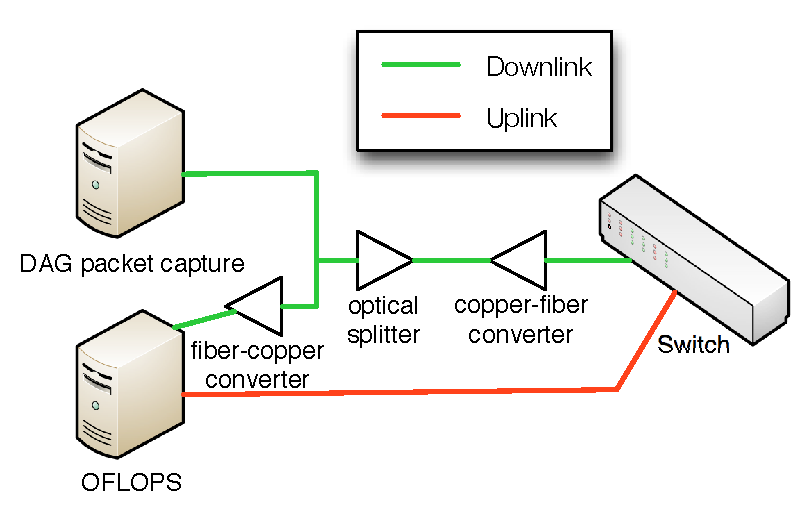
\includegraphics[width=0.99\textwidth]{Chapter1/Chapter1Figs/accuracy-topology} 
 \caption{\oflops precision evaluation topology against a DAG card.} 
 \label{fig:timestamping_topology}
\end{minipage}
\hspace{0.5cm}
  \begin{minipage}[b]{0.45\textwidth}
\centering
 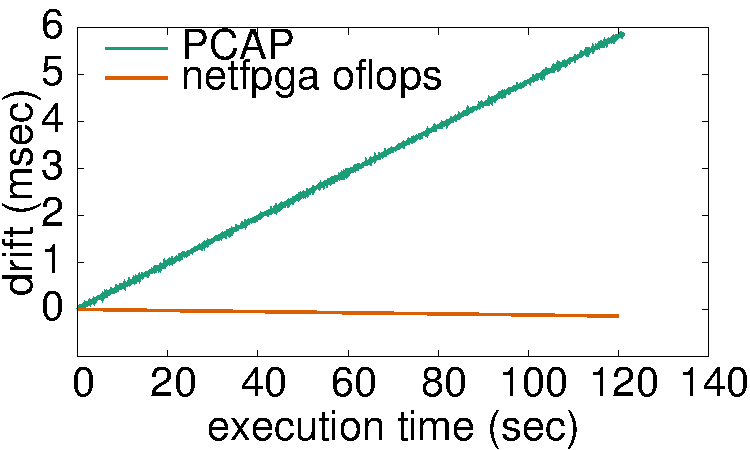
\includegraphics[width=0.99\textwidth]{Chapter1/Chapter1Figs/timer-precision} 
 \caption[Precision evaluation of PCAP and NetFPGA timestamps]{Timestamping
 precision evaluation using a DAG card. PCAP timestamps exhibit a significant
 drift in the order of microseconds, in comparison to the NetFPGA hardware
 design.}
\label{fig:timestamping}
\end{minipage}
\end{figure}

Figure~\ref{fig:timestamping_topology} presents a simple evaluation setup for
the accuracy of the \oflops capturing timestamps, in comparison to a DAG
card~\mycite{dag_card}. For the measurement, we use a 100 Mbps CBR probe of
small packets (90 bytes) for a two minute period. The probe is duplicated, using an optical
wiretap with negligible delay, and sent simultaneously to \oflops and to the DAG
card. In Figure~\ref{fig:timestamping}, we plot per-packet drift between each
\oflops timestamping mechanism and the DAG card. From the figure, we note that
the PCAP timestamps drift by 6 ms after 2 minutes, while the NetFPGA
timestamping mechanism exhibits lower drift on the order of microseconds.




\section{Measurement Setup}\label{sec:oflops-switches}

At the end of 2009, the \of specification was released in its first
stable version, 1.0~\mycite{openflow-spec}, the first recommended version
implemented by vendors for production systems.  Our analysis was conducted in
collaboration with T-labs in Spring of 2011. During that period, the
introduction of \of support in commodity switches was limited, and only a small
number of devices provided production-level support for the protocol.  Using
\oflops, we evaluated \of-enabled switches from three different switch vendors.
Vendor 1 provided production-ready \of support, whereas vendors 2 and 3 during
that period provided experimental \of support. The set of selected switches
provided a representative but not exhaustive sample of available \of-enabled
ToR-type switching hardware, during that time. Finally, we also include in our
measurement a recent \of switch which provides production support up
to version 1.1 of the protocol (firmware was released in December
2013).  Switch4 uses the \ovs codebase for its implementation. 
Table~\ref{tbl:switch_list} provides details regarding the CPU and the size of
the flow table for each switch. In addition, the switching fabric in the vendor
hardware specification reports similar non-blocking capacity and packet
processing rates. 

\of is not limited to hardware. The protocol reference implementation is the software
switch, \ovs~\mycite{openvswitch}, an important implementation for production
environments. Firstly, \ovs provides a replacement for the poor-performing Linux
bridge~\mycite{bianco10}, a crucial functionality for virtualised operating
systems.  Currently, the Xen platform uses \ovs to forward traffic between VMs
in the Dom0, a configuration which is inherited by major Cloud providers, like
Amazon and Rackspace.  Secondly, several hardware switch vendors use the \ovs
codebase for the development of their own \of-enabled firmwares. The \ovs development
team has standardised a clean abstraction for the control of packet
forwarding elements (similar to Linux HAL), which allows code reuse by any
forwarding entity. Thus, the mature software implementation of the \of protocol
is ported to commercial hardware, making certain implementation bugs less likely
to (re)appear.  We preclude \ovs in our performance and scalability study of
hardware switches. Finally, in our comparison we include the \of switch design
for the NetFPGA platform~\mycite{openflow-netfpga}. This implementation is based
on the original \of reference implementation~\mycite{of-reference-impl}, extending
it with a hardware forwarding design. 

\begin{table}[h!]
  \begin{center}
  \begin{tabular}{|c | c | c |}
    \hline                        
    \textbf{Switch} & \textbf{CPU} & \textbf{Flow table size} \\
    \hline  
    Switch1 & PowerPC 500MHz & 3072 mixed flows \\
    \hline  
    Switch2 & PowerPC 666MHz & 1500 mixed flows \\
    \hline  
    Switch3 & PowerPC 828MHz & 2048 mixed flows \\
    \hline  
    Switch4 & MIPS 1.1 SoC  & 2048 mixed flows \\
    \hline  
    \ovs & Xeon 3.6GHz & 1M mixed flows \\
    \hline  
    NetFPGA &  DualCore 2.4GHz & 32K exact \& 100 wildcard \\
    \hline 
  \end{tabular}  
\end{center}
\caption{OpenFlow switch details.}
\label{tbl:switch_list}
\end{table}

In order to conduct our measurements, we setup \oflops on a dual-core 2.4GHz
Xeon server equipped with a NetFPGA card.  For all of the experiments we utilized
the NetFPGA-based packet generating and capturing mechanism. 1 GbE control and
data channels are connected directly to the tested switches. We measured the
processing delay incurred by the NetFPGA-based hardware design to be a
near-constant $900$ ns.

\section{Switch Evaluation}\label{sec:oflops-result}

As for most networking standards, there are different ways to implement a given
protocol based on a paper specification. \of is no different in this regard. The
current \of reference implementation is \ovs~\mycite{openvswitch}. However,
different software and hardware implementations may not implement all features
defined in the \ovs reference, or they may behave in an unexpected way. In order
to understand the behaviour of an \of switch implementation, we developed a suite of
measurement experiments to benchmark the functionality of the elementary
protocol interactions.  These tests target: 
\begin{enumerate}
  \item The \of packet processing actions~(Section~\ref{sec:results-packets})
  \item The packet interception and packet injection functionality of the
        protocol~(Section~\ref{sec:results-pktin})
  \item The update rate of the flow table and its impact on the data
        plane,~(Section~\ref{sec:results-rate})
  \item The monitoring capabilities provided by
        \of~(Section~\ref{sec:results-monitoring})
  \item The impact of interactions between different \of
        operations~(Section~\ref{sec:results-interactions}).  
\end{enumerate}


\subsection{Packet Modifications}\label{sec:results-packets}

The \of 1.0 specification~\mycite{openflow-spec} defines 10 packet modification
actions which can be applied on incoming packets. Available actions include
modification of source and destination MAC and IP addresses, VLAN tag and PCP
fields and TCP and UDP source and destination port numbers. The action list
of a flow definition can contain any combination of them. The left column of
Table~\ref{tbl:feature_delay} lists the packet fields that can be modified by an
\of-enabled switch.  These actions are used by network devices such as IP
routers (e.g. rewriting of source and destination MAC addresses) and NAT
(rewriting of IP addresses and ports). Existing network equipment is tailored to
perform a subset of these operations, usually in hardware to sustain line rate.

To measure the time taken by an \of switch to modify a packet field header, we
generated from the NetFPGA card UDP packets of 100 bytes, at a constant rate of
100Mbps (approximately 125 Kpps).  This rate is high enough to give
statistically significant results in a short period of time, without introducing
packet queuing in software-based switches.  The flow table is initialized with a
flow that applies a specific action on all probe packets and the processing
delay is calculated as the difference between the transmission and receipt
timestamps provided by the NetFPGA card.  We report in
Table~\ref{tbl:feature_delay} the median processing delay for each action, along
with its standard deviation, and the percent of lost packets of the measurement
probe.

\begin{table*}[tb]
  \centering
  \begin{tabular}[t]{|l | c | c | c || c | c | c  || c | c | c |}
    \hline                       
    Mod. \ type & \multicolumn{3}{|c|}{Switch1} &
    \multicolumn{3}{|c|}{Switch2} & \multicolumn{3}{|c|}{Switch3} \\ \hline                       
              & med & sd & loss\%  & med & sd  & loss\% & med & sd & loss\%  \\ \hline  
    Forward   & 4  & 0   & 0       & 6   & 0   & 0      & 5   & 0  & 0       \\ \hline  
    MAC addr. & 4  & 0   & 0       & 302 & 727 & 88     & -   & -  & 100     \\ \hline  
    IP addr.  & 3  & 0   & 0       & 302 & 615 & 88     & -   & -  &  100    \\ \hline  
    IP ToS    & 3  & 0   & 0       & 6   & 0   & 0      & -   & -  & 100     \\ \hline  
    L4 port   & 3  & 0   & 0       & 302 & 611 & 88     & -   & -  & 100     \\ \hline  
    VLAN pcp  & 3  & 0   & 0       & 6   & 0   & 0      & 5   & 0  & 0       \\ \hline  
    VLAN id   & 4  & 0   & 0       & 301 & 610 & 88     & 5   & 0  & 0       \\ \hline  
    VLAN rem. & 4  & 0   & 0       & 335 & 626 & 88     & 5   & 0  & 0       \\ \hline
  \end{tabular}
  \begin{tabular}[t]{|l | c | c | c || c | c | c || c | c | c |}
    \hline                       
    Mod. \ type & \multicolumn{3}{|c|}{Switch4} & \multicolumn{3}{|c|}{\ovs} &\multicolumn{3}{|c|}{NetFPGA}\\ \hline                       
              & med & sd & loss\% & med & sd & loss\% & med & sd & loss\% \\ \hline  
    Forward   & 2   & 0  & 0      & 35  & 13 & 0      & 3   & 0  & 0      \\\hline  
    MAC addr. & 2   & 0  & 0      & 35  & 13 & 0      & 3   & 0  & 0      \\ \hline  
    IP addr.  & 2   & 0  & 0      & 36  & 13 & 0      & 3   & 0  & 0      \\ \hline  
    IP ToS    & 2   & 0  & 0      & 36  & 16 & 0      & 3   & 0  & 0      \\ \hline  
    L4 port   & 2   & 0  & 0      & 35  & 15 & 0      & 3   & 0  & 0      \\ \hline  
    VLAN pcp  & 2   & 0  & 0      & 36  & 20 & 0      & 3   & 0  & 0      \\ \hline  
    VLAN id   & 2   & 0  & 0      & 35  & 17 & 0      & 3   & 0  & 0      \\ \hline  
    VLAN rem. & 2   & 0  & 0      & 35  & 15 & 0      & 3   & 0  & 0      \\ \hline
  \end{tabular}
 
  \caption[Switch action latency.]{Time in $\mu$s to perform individual packet
    modifications and packet loss. Processing delay indicates whether the
    operation is implemented in hardware (\textless10$\mu$s) or performed by
    the CPU (\textgreater10$\mu$s).}
  \label{tbl:feature_delay}
\end{table*}

We observe significant differences in the performance of the hardware switches
due in part to the way their firmware implements packet modifications. Switch1
and Switch2, with their production-grade implementations, handle all
modifications in hardware; this explains their low packet processing delay of
between 2 and 4 $\mu$s. On the other hand, Switch2 and Switch3 each run
experimental firmware that provided, at the time, only partial hardware support
for \of actions. Switch2 uses the switch CPU to perform some of the available
field modifications, resulting in processing delay and variance two orders of
magnitude higher packet.  Switch3 follows a different approach; all packets of
flows with actions not supported in hardware are silently discarded. The
performance of the \ovs software implementation lies between Switch1 and the
other hardware switches.  \ovs fully implements all \of actions. However,
hardware switches outperform \ovs as the flow actions are supported in
hardware. Finally, the NetFPGA design provides support for all actions in
hardware and allows line rate support with low and constant processing latency. 

We conducted a further series of experiments with variable numbers of packet
modifications in the flow action list. We observed, that the combined processing
time of a set of packet modifications is equal to the highest processing time
across all individual actions in the set (e.g.~Switch2 required approximately
300~ms per packet to modify both IP source addresses and IP ToS field).
Furthermore, we noticed that Switch1, Switch4 and \ovs have a limit of 7
actions, which exposes limits enclosed in the implementation.

\subsection{Traffic Interception and Injection}\label{sec:results-pktin}

\begin{figure}[t]
  \begin{center}
    \subfigure[{\tt pkt\_in} processing latency]
    {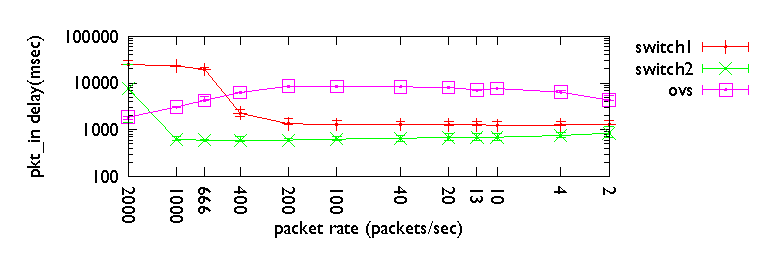
\includegraphics[width=0.99\textwidth]{Chapter1/Chapter1Figs/pkt_in_delay}\label{fig:pkt_in_delay}}
    \subfigure[{\tt pkt\_out} processing latency]
	{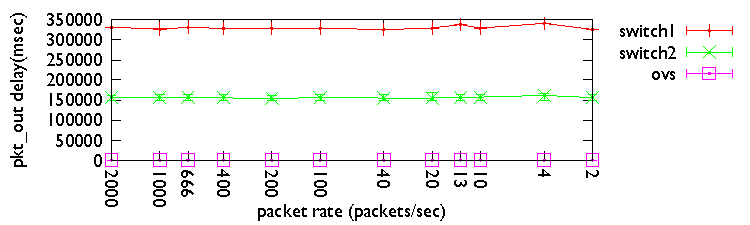
\includegraphics[width=0.99\textwidth]{Chapter1/Chapter1Figs/pkt_out_delay}\label{fig:pkt_out_delay}}
  \end{center}
  \caption[\texttt{pkt\_in} and \texttt{pkt\_out} processing latency]{Latency to
    intercept (Figure~\ref{fig:pkt_in_delay}) and inject
    (Figure~\ref{fig:pkt_out_delay}) data plane packets using the \of protocol.}
  \label{fig:pkt_in_out_delay}
\end{figure}

\of protocol permits a controller to intercept or inject traffic through the
control plane. Packet interception is fundamental for reactive control, while
packet injection enables applications to interact with data plane end-hosts and
devices, e.g.~topology discovery using the LLDP protocol.  In order to
characterise the performance of these functionalities, we conducted two
experiments.  The first experiment invalidates all flow table entries and uses a
data plane probe of small packets (100 bytes) on a data channel to  measure the
per-packet delay between the packet transmission and its reception on the
control plane, as a \texttt{pkt\_in} message. The second experiment generates a
control plane probe using \texttt{pkt\_out} messages and measures the delay in
receiving each packet on a data channel.  

Figure~\ref{fig:pkt_in_out_delay} presents the $10_{th}$, $90_{th}$ percentiles and
median per-packet processing latency for varying probe rates. We omitted Switch3 in
this experiment, because these functionalities incurred significant co-processor
load, resulting in control plane unresponsiveness.  In terms of packet
injection, hardware switches exhibit high latency (150 ms for Switch2 and 350
ms for Switch1), in comparison to \ovs and Switch4 (approximately 0.1 ms).
For hardware switches, we noticed at high packet rates that packet
transmissions were rate-limited using the advertised window of the control plane
TCP connection. In terms of traffic interception, we observed diverse behaviours
between hardware switches at high packet rates. For Switch1, latency becomes
note-worthy beyond 400 packets/second, resulting in a median latency of 1 ms,
while the switch can process up to 500 packets/second, with median latency of 10
ms. For Switch2, latency is significantly lower, with a median value of
800~$\mu$s and reaches 10 seconds only when the probe rate is 2,000
packets/second. Switch4 exhibits a constant delay, between 9 and 17 ms, but the
packet rate is limited to 50 packets/second.  \ovs, has a high but stable latency,
between 1 and 10 ms, for any tested data rate. 

\subsection{Flow Table Update Rate}\label{sec:results-rate}

The flow table is a central component of an \of switch and is the equivalent of
a Forwarding Information Base (FIB) on routers. Given the importance of FIB
updates on commercial routers, e.g. to reduce the impact of control plane
dynamics on the data plane, the FIB update processing time of commercial routers
provides useful reference points and lower bounds for the time to update a flow
entry on an \of switch. The time to install a new entry on commercial routers
has been reported in the range of a few hundreds of
microseconds~\mycite{shaikh-igp}.

\of has a mechanism for defining barriers between sets of commands: the
\texttt{barrier} command. According to the \of
specification~\mycite{openflow-spec}, the \texttt{barrier} command is a way of being
notified that a set of \of operations has been completed. Furthermore, the switch
has to complete the set of operations issued prior to the \texttt{barrier}
before executing any further operation. If the \of implementations comply with
the specification, we expect to receive a \texttt{barrier} notification for a
flow modification once the flow table of the switch has been updated, implying
that the change can be seen from the data plane.

We checked the behaviours of the tested \of implementations, finding variation among
them. For \ovs, and Switch1, Figure~\ref{fig:flow_insertion_comparison} shows the
time to install a set of entries in the flow table. Switch2 and Switch3 are not
reported, as this \of message is not supported by the firmware.  For this
experiment, \oflops worked on a stream of packets of 100 bytes at a constant
rate of 100 Kpackets/second (10 Mbps) that targeted the newly installed flows in a
round-robin manner. The probe achieved sufficiently low inter-packet periods in
order to accurately measure the flow insertion time.

\begin{figure}[h]
  \centering
    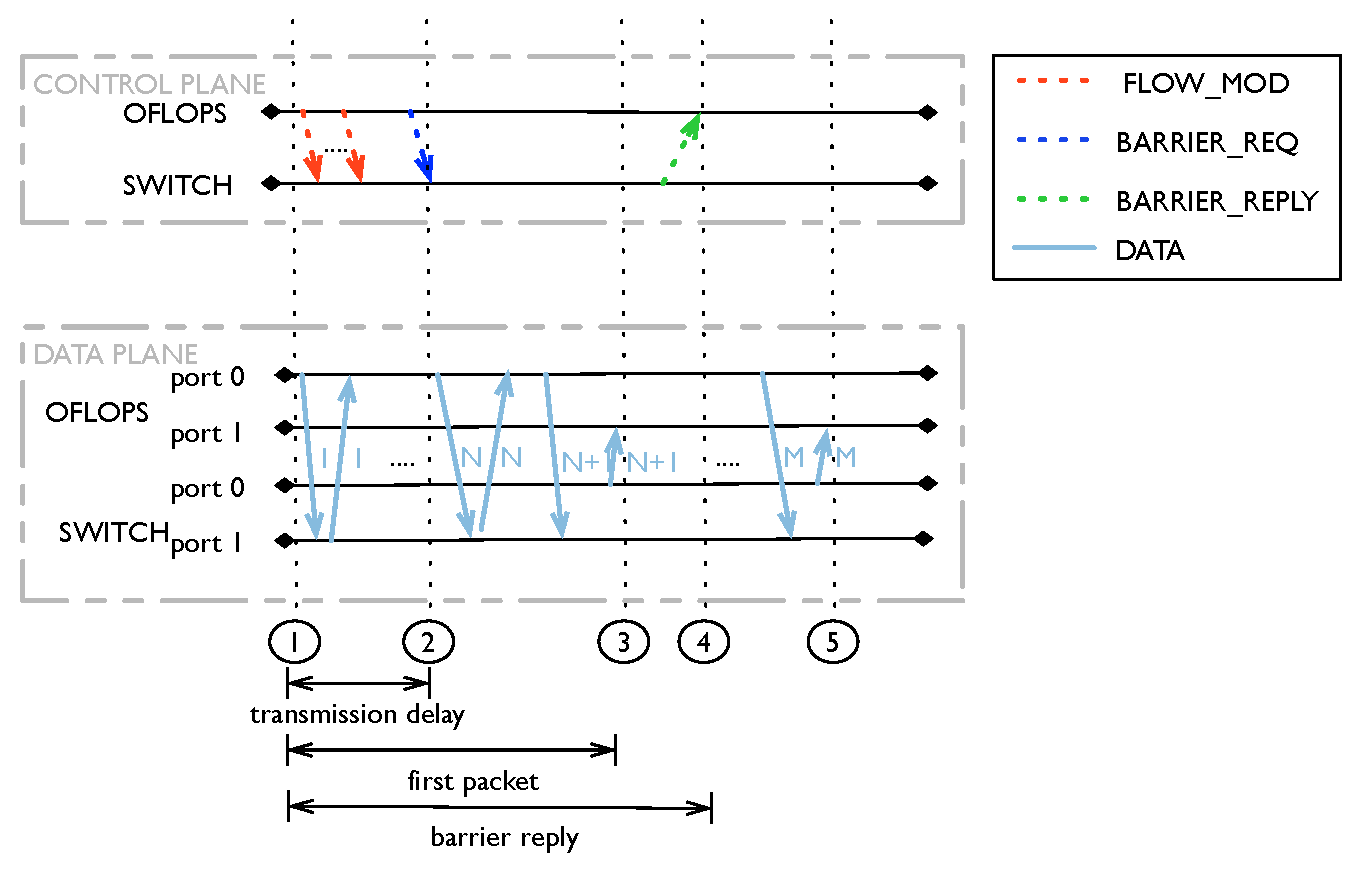
\includegraphics[width=0.99\textwidth]{Chapter1/Chapter1Figs/flow_insertion_seq_diagram} 
    \label{fig:flow_mod_scenario}
    \caption[Flow insertion and flow modification measurement scenario] {Flow 
    insertion and flow modification measurement scenario. The experiment uses
    multiple information channels to estimate the delay in modifying entries in
    the flow table.}
\end{figure}

\begin{figure}[ht]
  \begin{center}
    \subfigure[\ovs (log-log scale)]
    {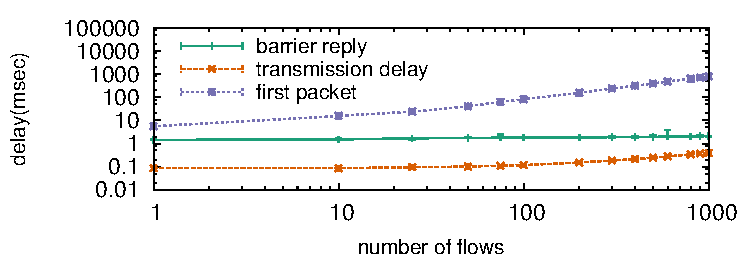
\includegraphics[width=0.99\textwidth]{Chapter1/Chapter1Figs/openvswitch_mod_flow_exact_comparison}}
    \subfigure[Switch1 (log-log scale)]
	{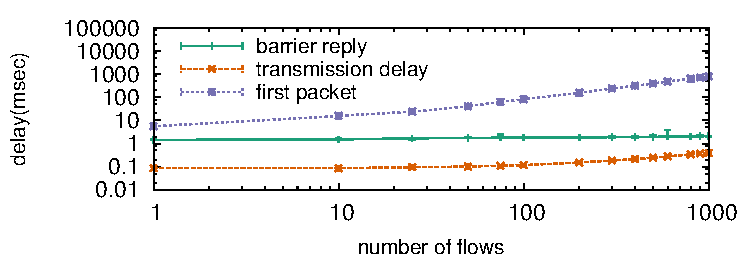
\includegraphics[width=0.99\textwidth]{Chapter1/Chapter1Figs/switch1_mod_flow_exact_comparison}}
  \end{center}
  \caption[Flow entry insertion delay]{Flow entry insertion delay: as reported using the
    \texttt{barrier} notification and observed at the data
    plane.}
  \label{fig:flow_insertion_comparison}
\end{figure}


Figure~\ref{fig:flow_mod_scenario} presents the measurement scenario,
while~\ref{fig:flow_insertion_comparison} presents three different measured
latencies.  The first, {\it barrier reply} is derived by measuring the
time elapsed between when the \textbf{first insertion command} is sent by the \oflops
controller and the time the \texttt{barrier} reply is received by the
PC\@. The second, {\it transmission delay}, is the time elapsed between when the first and
last flow insertion commands are sent out from the PC running \oflops.  The
third, {\it first packet}, is the time elapsed between when the \textbf{first insertion
  command} is issued and when a packet has been observed for the last of the (newly)
inserted rules. For each configuration, we ran the experiment 100 times and
Figure~\ref{fig:flow_insertion_comparison} shows the median result as well as
the $10^{th}$ and $90^{th}$ percentiles, although the variations are small and
cannot be easily viewed.

From Figure~\ref{fig:flow_insertion_comparison}, we observe that even though the
\textit{transmission delay} in sending flow insertion commands increases
proportionally to the flow number, this time is negligible when compared with
data plane measurements (\textit{first packet}). Notably, the \textit{barrier
  reply} measurements are almost constant, increasing only as the
transmission delay increases (difficult to discern on the log-log plot) and,
critically, this operation returns before any \textit{first packet} measurement.
This implies that the way the \textit{barrier reply} is implemented does
not reflect the time when the hardware flow-table has been updated.

These results demonstrate how \oflops computes per-flow overheads. We
observed that the flow insertion time for Switch1 starts at $1.8$ ms for a single
entry, but converges toward an approximate overhead of $1$ ms per inserted entry
as the number of insertions grows.

\subsubsection*{Flow insertion types}

\begin{figure}[h]
  \begin{center}
    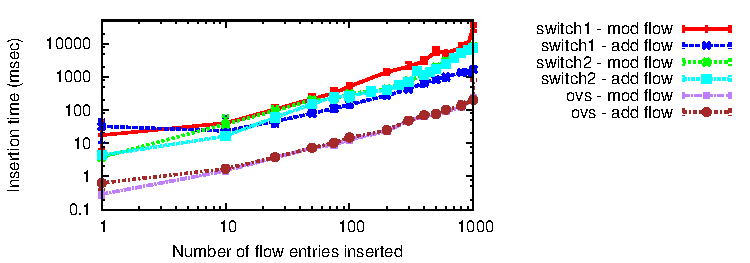
\includegraphics[width=0.99\textwidth]{Chapter1/Chapter1Figs/flow_insertion_delay}
  \end{center}
  \caption[Delay of flow insertion and flow modification]{Delay of flow insertion 
  and flow modification, as observed from the data plane (log-log scale).}
  \label{fig:flow_insertion_delay}
\end{figure}

We now distinguish between flow insertions and the modification of existing
flows.  With \of, a flow rule may perform exact packet matches or use
wildcards to match a range of values. Figure~\ref{fig:flow_insertion_delay}
measures the flow insertion delay as a function of the number of inserted
entries. This is done for the insertion of new entries and for the modification
of existing entries.

These results show that for software switches that keep all entries in memory,
the type of entry or insertion does not make a difference in the flow insertion
time.  Surprisingly, both Switch1 and Switch2 take more time to modify existing
flow entries compared to adding new flow entries.  For Switch1, this occurs for
more than 10 new entries, while for Switch2 this occurs after a few tens of new
entries.  After discussing this issue with the vendor of Switch2, we came to the
following conclusion: as the number of TCAM entries increases, updates become
more complex as they typically require re-ordering of existing entries.
\mycitet{Gupta01} characterise the update complexity of a TCAM as linear.

Clearly, the results depend both on the entry type and implementation.  For
example, exact match entries may be handled through a hardware or software hash
table. Whereas wildcarded entries, requiring support for variable length
lookup, must be handled by specialized memory modules, such as a TCAM\@. With such
possible choices and a range of different experiments, the flow insertion times
reported in Figure~\ref{fig:flow_insertion_delay} are not generalizable, but
rather depend on the type of insertion entry and implementation.

\subsection{Flow Monitoring}\label{sec:results-monitoring}

The use of \of as a monitoring platform has already been suggested for the
applications of traffic matrix computation~\mycite{opentm-pam,tm-presto} and
identifying large traffic aggregates~\mycite{openflow-measurement-hotice}. To
obtain direct information about the state of the traffic received by an \of
switch, the \of protocol provides a mechanism to query traffic statistics,
either on a per-flow basis or across aggregates matching multiple flows and
supports packet and byte counters. 

We now test the performance implications of the traffic statistics reporting
mechanism of \of. Using \oflops, we installed flow entries that match packets sent
on the data path. Simultaneously, we started sending flow statistics requests to
the switch. Throughout the experiment we recorded the delay in getting a reply for
each query, the amount of packets that the switch sends for each reply, and the
departure and arrival timestamps of the probe packets.

Figure~\ref{fig:stat_request_latency} reports the time taken to receive a flow
statistics reply for each switch as a function of the request rate. Despite the
rate of statistics requests being modest, quite high CPU utilization is recorded
for even a few queries per second being sent. Figure~\ref{fig:stat_request_cpu}
reports the switch-CPU utilization as a function of the flow statistics
inter-request time. Statistics are retrieved using SNMP\@. Switch3 is excluded for
lack of SNMP support.

\begin{figure}[h]
  \begin{center}
    \subfigure[Reply time.]
    {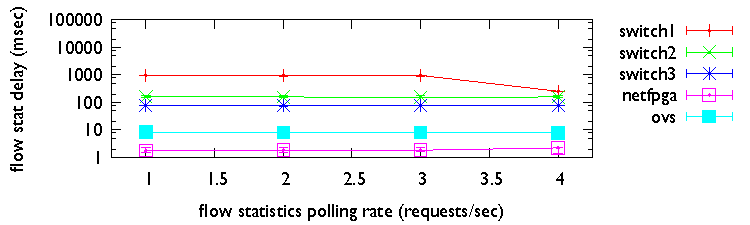
\includegraphics[width=0.99\textwidth]{Chapter1/Chapter1Figs/flow_stats_delay} \label{fig:stat_request_latency}}
    \subfigure[CPU utilization.]
      {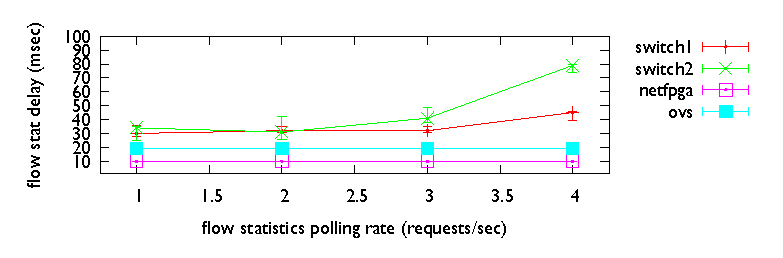
\includegraphics[width=0.99\textwidth]{Chapter1/Chapter1Figs/flow_stats_cpu}\label{fig:stat_request_cpu}}
  \end{center}
  \caption{Time to receive a flow statistic (median) and corresponding CPU utilization.}
  \label{fig:stat_request}
\end{figure}

From the flow statistics reply times, we observe that all switches have
(near) constant response delays; the delay itself relates to the type of switch.
As expected, software switches have faster response times than hardware
switches, reflecting the availability of the information in memory without the
need to poll multiple hardware counters. These consistent response times also
hide the behaviour of the exclusively hardware switches, whose CPU time increases
proportionally with the rate of requests.  We observe two types of behaviour from
the hardware switches: the switch has a high CPU utilization, answering
\texttt{flow\_stats} requests as fast as possible (Switch2); or the switch delays
responses, avoiding over-loading its CPU (Switch1). Furthermore, for Switch1, we
noticed that the switch is applying a pacing mechanism on its replies.
Specifically, at low polling rates the switch splits its answer across multiple
TCP segments, each segment containing statistics for a single flow.  As the
probing rate increases, the switch will aggregate multiple flows into a single
segment. This suggests that independent queuing mechanisms are used for handling
flow statistics requests. Finally, neither software nor NetFPGA switches see an
impact of the \texttt{flow\_stats} rate on their CPU, thanks to their significantly more
powerful PC CPUs (Table~\ref{tbl:switch_list}).

%%%%%%%%%%%%%%%%%%%%%%%%%%%%%%%%%%%%%%%%%
\subsection{\of Command Interaction}\label{sec:results-interactions}
%%%%%%%%%%%%%%%%%%%%%%%%%%%%%%%%%%%%%%%%%

% why is it important this experiment

An advanced feature of \of is its ability to provide network
control applications with, for example, flow arrival notifications from the network,
while simultaneously providing fine-grain control of the forwarding process.
This permits applications to adapt in real time to the requirements and load of
the network~\mycite{handigol09,Yap09}. Using \oflops measurement
instrumentation, we developed a test scenario of dynamic network control, in order
to understand the behaviour of the switch control and data plane.  In this
scenario, we emulated the simultaneous querying of traffic statistics and
modification of the flow table.  More specifically, we extended
Section~\ref{sec:results-rate} by showing how the mechanisms of traffic
statistics extraction and table manipulation interact. Specifically, we
initialized the flow table with 1024 exact match flows and measured the delay to
update a subset of 100 flows.  Simultaneously, the measurement module polls the
switch for full table statistics at a constant rate. The experiment uses a
constant rate 10 Mbps packet probe to monitor the data path, and polls every 10
seconds for SNMP CPU values.

\begin{figure}[t]
  \begin{center}
    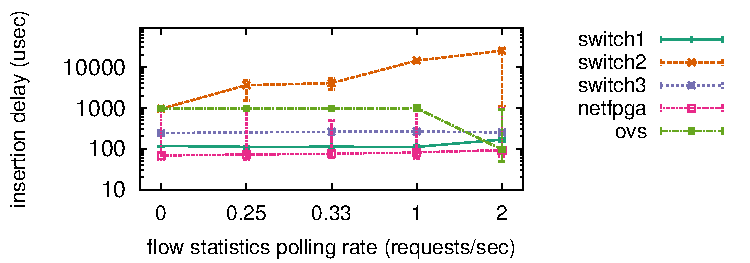
\includegraphics[width=0.99\textwidth]{Chapter1/Chapter1Figs/interaction_test}
  \end{center}
  \caption{Delay when updating  flow table while the controller polls
    for statistics.}
  \label{fig:interaction_test}
\end{figure}

In this experiment, we controlled the probing rate for the flow statistics
extraction mechanism, and we plotted the time necessary before the modified flows
become active in the flow table. For each probing rate, we repeated the experiment
50 times, plotting the median, $10^{th}$ and $90^{th}$ percentile. In
Figure~\ref{fig:interaction_test} we can see that, for lower polling rates,
implementations have a near-constant insertion delay comparable to the results
of Section~\ref{sec:results-rate}.  For higher probing rates on the other hand,
Switch1 and Switch3 do not differ much in their behaviour. In contrast, Switch2
exhibits a noteworthy increase in the insertion delay. This is explained by the
CPU utilization increase incurred by the flow statistics polling
(Figure~\ref{fig:stat_request_cpu}). Finally, \ovs has a marginal decrease
in the median insertion delay, and at the same time an increase in its variance.
We believe that this behaviour is caused by interactions with the OS scheduling
mechanism: the constant polling causes frequent interrupts for the user-space
daemon of the switch, which leads to a batched handling of requests.

\section{Network Control Macro-experimentation} \label{sec:sdnsim-intro}

\oflops and Cbench~\mycite{cbench} provide a sufficient toolbox for profiling the
building blocks of \of, the switch and the controller.  Nonetheless, in order to
understand the impact of a control architecture, we require
mechanisms that transform \of performance models into network-wide measurements
under specific traffic patterns and network topologies.  A popular approach to
examine performance and correctness uses experimental setups which
reproduce specific network-wide functionalities.  Network experimentation uses
two primary approaches: \textit{emulation} and \textit{simulation}.

Network emulation scales network system behaviour replication by replacing
portions of network functionality with simpler models.  \mycitet{Vahdat2002}
present Modelnet, an early network emulation framework attempt, which used
highly optimized in-kernel resource control primitives to simulate large
Internet-scale systems. Recent efforts employ lightweight virtualisation to
scale large-scale network experiments~\mycite{Handigol12b,Puljiz06,Gupta2011}.
Network emulation approaches provide an effective solution to network
experimentation, but the experimental fidelity is bound by the computational
resources of the execution environment.

A notable approach to network emulation employs real testbeds to reproduce in
full detail an experiment, and achieve maximum fidelity. Real testbeds incur
significant resource and configuration overhead, which scale sub-linearly with
respect to the size of the experiment. In an effort to improve resource
scalability, the research community builds and maintains a series of shared
testbeds, which multiplex experimental deployments in shared infrastructure
using virtualisation~\mycite{planetlab,ofelia}.  Shared testbeds fulfil the
requirements for a wide range of experiments, but the resource sharing
techniques limit measurement precision~\mycite{Kim11b}, as they introduce noise which is not
always detectable and removable.

Network simulation replaces network functionality with simplified
models~\mycite{Varga2008,issariyakul2012}.  Simulation platforms set out to
provide good resource scalability, but ultimately the accuracy and scalability
is influenced by the assumptions of the network models and implementation.  In
addition, the programming abstractions in simulation platforms remain
extensively incompatible with real system programming abstractions and, as a
result, require a significant effort to transfer functionality between the two
domains.  For example, POSIX socket-based applications must modify their
connection abstraction to match the API of the simulation platform, while
forwarding plane traffic patterns may have to transform into stochastic models. 

Network simulation and emulation follow two philosophically distinct approaches
to scale experiments, each providing different trade-offs.   In the section, we
present \sdnsim\footnote{\sdnsim is under the GPL licence and can be downloaded
  from \url{http://github.com/crotsos/sdnsim/}}, a network experimentation
framework which bridges the two aforementioned approaches. The framework is
written in OCaml, a high performance functional language, and extends the
functionality of the Mirage\footnote{\mirageurl} library OS\@.  Experimenters can
describe network functionality over the \mirage OS systems API, and, during
compilation, transform the experimental definition into a concrete experiment
realisation. \sdnsim provides two experimentation options: \emph{Simulation},
transforms the experiment definition into an \ns{3}~\mycite{Henderson2006}
simulation, and \emph{Emulation}, emulates the experiment definition using 
the Xen virtualisation platform~\mycite{Barham2003}.

\section{Network Experimentation} \label{sec:experimentation}

This section presents the design of the \sdnsim platform.  We
present the \mirage library OS (Section~\ref{sec:mirage-intro}), a core building
block for the functionality of experimentation nodes, and
elaborate on the functionality of \sdnsim and its integration with
the \ns{3} and Xen platform (Section~\ref{sec:sdnsim-design}). 

\subsection{Mirage Library OS} \label{sec:mirage-intro}

\begin{table}
\centering
\begin{tabular}{@{\extracolsep{0pt}}l|c}
\emph{Appliance} & \emph{Binary size (MB)} \\ 
\hline
DNS & 0.184 \\
Web Server & 0.172 \\
\of switch & 0.164 \\
\of controller & 0.168 \\
\end{tabular}
\caption[Sizes of Mirage application images.]{\label{t:codesize}Sizes of Mirage
application images. Configuration and data are compiled directly into the
image.}
\end{table}

Mirage~\mycite{madhavapeddy2013} is a development framework for cloud services,
supporting the transformation of applications in single purpose appliances,
compile-time specialised into stand-alone Xen-compliant kernels.  \sdnsim
re-uses the Mirage abstraction and code to develop host functionality for two core
reasons: the low memory footprint of Mirage applications; and its clean and
simplified design. Mirage revisits the idea of library OS; functionality is
separated into logical modules and linked to an appliance only if the code
expresses an explicit dependency.  As a result, Mirage by design results in
compact OS images with very low memory requirements.  Table~\ref{t:codesize}
presents the compiled image size for a set of Mirage applications.

Mirage OS exposes a simple systems programming API, implemented by two core
modules: \textit{Net} and \textit{OS}.  The OS module provides thread
scheduling, device management and IO functionality, while the Net module
provides a network stack supporting ICMP, IP, TCP, UDP and DHCP protocols. The
interface of the core Mirage API is sufficiently generic to enable development
of complex distributed services, while the OS architecture is sufficiently
simple and portable over a wide range of platforms.  Specifically, a Mirage
application can compile into a Xen image, a Linux application or a NodeJS
executable.  Currently, the platform is being ported to the FreeBSD kernel and
the BareMetal OS~\mycite{baremetalOS}, a high performance assembly-code OS.
Furthermore, Table~\ref{t:facilities} presents the wide range of network
protocols readily available in Mirage.

\subsection{\sdnsim Architecture} \label{sec:sdnsim-design}

\lstset{language=XML,
numberstyle=\footnotesize,
basicstyle=\ttfamily\footnotesize,
captionpos=b,
}
\begin{lstlisting}[caption={A sample \sdnsim configuration file interconnecting
  a server and a client host},label={lst:sdnsim-conf}]
<?xml version="1.0" encoding="ISO-8859-1"?>
<topology module="Simple_tcp_test" backend="ns3-direct" 
    slowdown="2.0" duration="30">
  <modules>
    <library>lwt</library>
    <library>lwt.syntax</library>
    <library>cstruct</library>
    <library>cstruct.syntax</library>
    <library>mirage</library>
    <library>mirage-net</library>
    <library>pttcp</library>
  </modules>
  <node name="host1" main="host_inner"> 
    <param>1</param>
  </node>
  <node name="host2" main="host_inner"> 
    <param>2</param>
  </node>
  <link src="host1" dst="host2" delay="10" rate="100" 
    queue_size="100" pcap="false"/>
  <link_ext host="host1" dev="eth1" delay="10" rate="100" 
    queue_size="100" pcap="false" ip="10.1.1.1">
</topology>
\end{lstlisting}

From the experimenter perspective, \sdnsim is an alternative build system for
\mirage applications. Experimenters implement host functionality as \mirage
applications and describe network topology using an XML-based configuration
file. \sdnsim is responsible for compiling the Mirage applications and
deploying the experiment, according to the configuration file. 

Listing~\ref{lst:sdnsim-conf} presents an \sdnsim configuration file for a
client (host1) - server (host2) architecture.  A minimal experimental
configuration consists of the name of the main OCaml module containing the host
code (topology@module), the target experimentation environment
(topology@backend) and the experiment duration (topology@duration).
Optionally, the emulation backend supports a slowdown parameter
(topology@slowdown) which controls a time dilation mechanism, presented in
detail in Section~\ref{sec:sdnsim:xen-backend}.  Hosts are defined using a
\texttt{host} XML entity, containing a host name (node@name), its main function
(node@main) and a variable number of children \texttt{param} entities
(node/param) for host initialisation.  Network link definitions use a
\texttt{link} XML entity, containing the name of the interconnected hosts
(link@src, link@dst), the device queue size (link@queue\_size), the link
propagation properties (link@rate, link@delay) and logging (link@pcap).
Finally, experiments can import external network interfaces, allowing
interaction with external applications.  Links with external hosts are defined
using a \texttt{link\_ext} XML entity, which has the same parameters as the
\texttt{link} entity, except from the \texttt{src} and \texttt{dst} attributes.
These attributes are replaced by the host (link\_ext@host) and dev
(link\_ext@dev) attributes, which map the network device of a host in the
experiment to a TUN/TAP network device. In addition, the optional IP
(link\_ext@ip) attribute defines the address and netmask of the TUN/TAP device. 

\begin{table}
\centering
\begin{tabular}{r|p{0.6\columnwidth}}
\emph{Subsystem} & \emph{Implemented Protocols} \\
\hline 
Network     & Ethernet, ARP, DHCP, IPv4, ICMP, UDP, TCP, \of\\ 
Storage     & Simple key-value, FAT-32, Append B-Tree, Memcache \\
Application & DNS, SSH, HTTP, XMPP, SMTP  \\ 
Formats     & JSON, XML, CSS, S-Expressions\\
\end{tabular}
\caption{\label{t:facilities}System facilities provided as \mirage{}
        libraries.}
\end{table}

\begin{figure}[ht] 
\centering
\subfigure[\ns{3}]{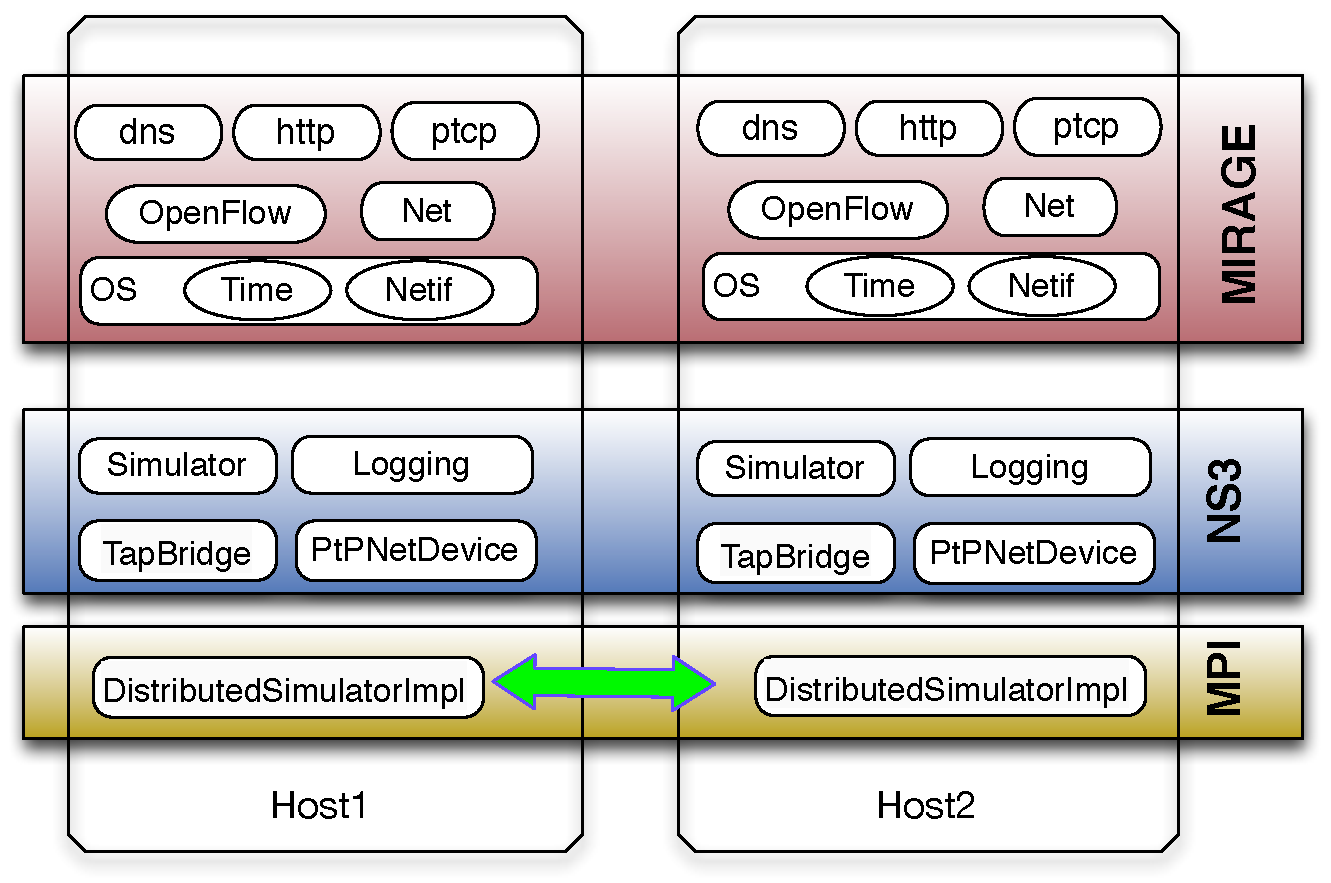
\includegraphics[width=0.45\textwidth]{Chapter1/Chapter1Figs/sdnsim-arch-ns3}\label{fig:sdnsim-arch-ns3}}
\subfigure[Xen] {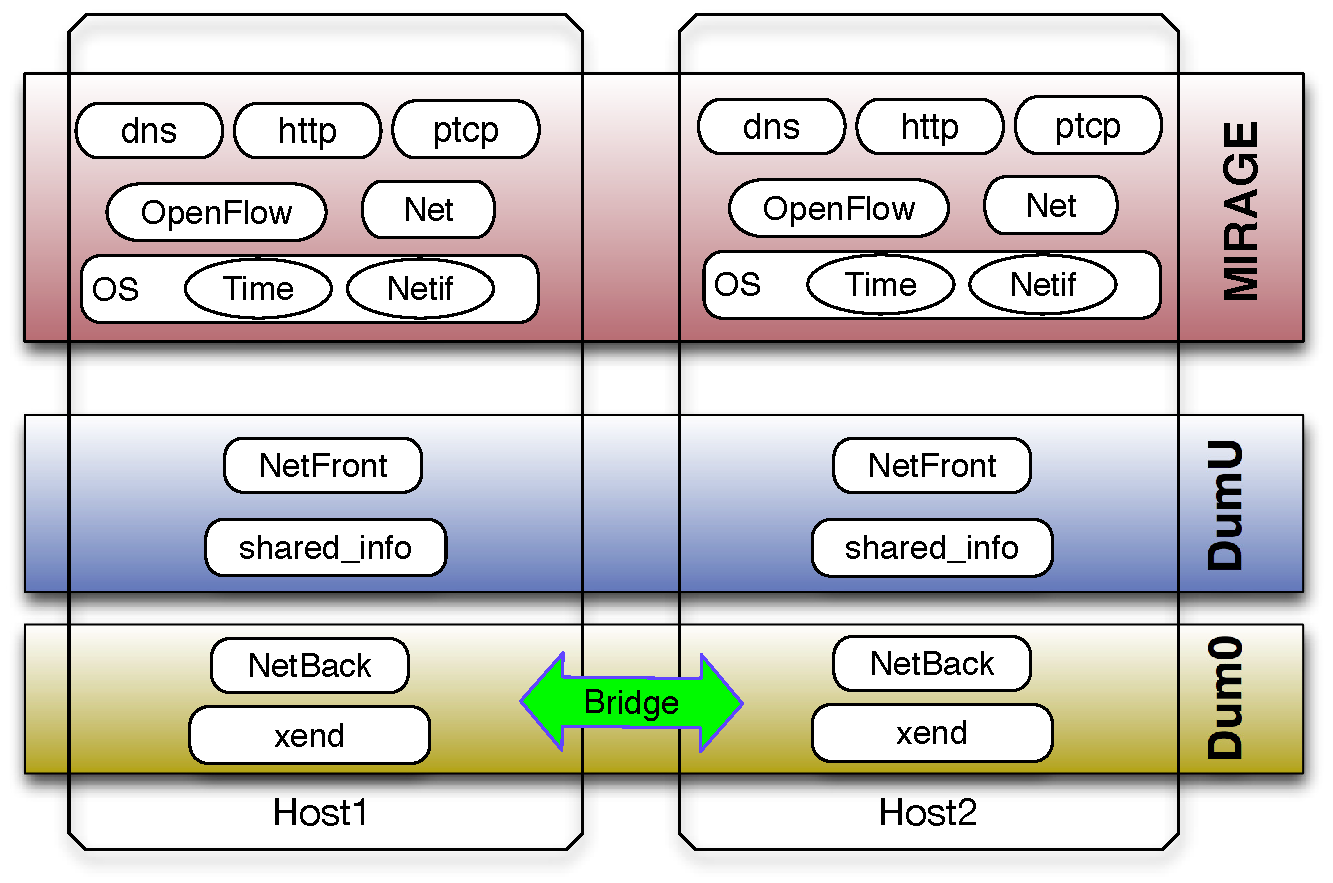
\includegraphics[width=0.45\textwidth]{Chapter1/Chapter1Figs/sdnsim-arch-xen}\label{fig:sdnsim-arch-xen}}
\caption[\sdnsim host internal architecture]{\sdnsim host internal architecture: \ns{3}
  simulation (Figure~\ref{fig:sdnsim-arch-ns3}) and Xen real-time
  emulation (Figure~\ref{fig:sdnsim-arch-xen}).}
\label{fig:sdnsim-arch}
\end{figure}


Figure~\ref{fig:sdnsim-arch} presents the host architecture in of \sdnsim
nodes. Host functionality is separated in three layers.  The top layer contains
the application logic of the host. This layer is defined by the experimenter,
and encodes the end-host network functionality. \sdnsim uses all application
libraries of the \mirage platform, enumerated in Table~\ref{t:facilities}, and
thus provides high traffic realism.  Furthermore, we extended the
ocaml-openflow library to incorporate switch and controller performance models
and implement the pttcp~\mycite{pttcp} traffic generator functionality in
OCaml, to support stochastic traffic models.  The middle layer of the host
architecture contains the core Mirage libraries and provides OS functionality
to the application layer. Finally, the lower layer of the host architecture,
provides integration between the Mirage OS and the execution backend.
Currently, \sdnsim has two experimentation backends: the \textit{\ns{3}}
simulation platform  and the \textit{Xen} virtualisation platform. These two
execution environments are highly heterogeneous and employ different execution
models. For the rest of this section, we present the integration details
between Mirage and each experimentation backend.  SNDSIM's main goal is network
accuracy and the presentation focuses on the network and time subsystems.

\subsubsection{Xen Backend} \label{sec:sdnsim:xen-backend}

\sdnsim uses the Xen virtualisation platform to emulate experimental
definitions. Hosts are represented as Mirage VMs, while network links are
realised using virtual interfaces (VIF) bridged in Dom0. \sdnsim replicate
network link properties using the resource control primitive (e.g.~throughput)
of the XEN VIF implementation.

Experiment setup uses the Xen Management API (XAPI)~\mycite{xapi}, which
provides an API to control programmatically the creation of VM instances and
VIFs. Specifically, the execution pipeline for an emulated experiment is the
following: host definitions are compiled in VM images, equivalent VM
configuration are created on Xen and network links are translated into
equivalent VIF and bridge setups. Once all configurations are completed,
created VMs are booted and experimentation scenario is executed for a
predefined duration.

As discussed in the previous section, a core limitation of experimental
emulation is computation resource scalability. In order to address this
problem,  \sdnsim modifies the Mirage core libraries to support time dilation
functionality.  Specifically, when the resources of the execution host are
insufficient, the experimenter can use a time dilation factor (TDF) to trade
time for resource scalability. Time dilation slows down time progression
synchronously across the emulated nodes, thus increasing the available resource
in a time unit. For example, a TDF value of 2 means that 1 second of emulation
time requires 2 seconds of real time to execute, doubling effectively the
experimental perceived CPU and network resources. Similar approaches have been
proposed in the domain of experimental emulation, in an effort to scale the
complexity of large topologies.  \mycite{Gupta2011} present a series of
modifications in the Xen hypervisor, providing time virtualisation.

The clean design of the \mirage OS provides easy modification of the time
subsystem. \mirage thread functionality relies on OCaml Lwt language extension,
an event-driven asynchronous programming library.  Lwt threads are cooperative
and non pre-emptive, either executing code or idling waiting for an IO event or a
synchronisation primitive (e.g.~a semaphore) or a timer event. The main thread
scheduler logic works as follows: Execute any resumable sleeping threads,
calculate the time left until the next timer event and poll the IO event channel
until that time expires. \sdnsim time virtualisation functionality requires only
a multiplication of the time events and time sources with the TDF value.  Guest
hosts access time information through a shared page with the hypervisor
containing a shared\_info struct containing CPU time information. Mirage
encapsulates access to the shared\_info page through a single \texttt{time}
function, which was modified with the TDF parameter. Similarly, we modify the
time event registration method to use the TDF parameter. Finally, time
virtualisation is enforced on network resources by dividing link throughput
values and multiplying link latency values with the TDF parameter. 

\subsubsection{\ns{3} Backend}

\sdnsim uses \ns{3}~\mycite{Henderson2006}, a discrete-time packet-driven network
simulator. The core of the system consists
of a time simulation engine, while the code base provides multiple libraries
modelling functionalities like network applications, routing protocols,
data-link layer protocols and link propagation models. \ns{3} is fundamentally
an extensive refactor of the \ns{2} code base, providing a stabler development
environment. 

The \ns{3} backend has a significant difference from the Xen backend; the
execution model is discrete and non-reentrant. \ns{3} applications register
their interest for specific time and network events, event handling is atomic
and the progress of the simulation is centrally controlled by the simulation
engine. In order to port Mirage to the \ns{3} simulation engine, we transformed
thread blocking calls into equivalent \ns{3} events.  More specifically, the
Mirage OS clock abstraction is bridged with the \ns{3} simulation clock and all
sleep calls are scheduled as \ns{3} time events.  A thread is resumed from a
sleep call when the simulator executes the respective time event.  Network
blocking calls are integrated with the network device abstraction of \ns{3}.
The packet reading thread registers a packet handler on the network device,
while the packet writing thread checks the device queue occupancy and blocks
when the queue is full. Finally, in order to avoid scheduling deadlocks, the OS
schedules {\it idle} \/time events to resume any yielded threads. Using these
transformations we are able to provide a semantically accurate integration of
\mirage with the \ns{3} engine.  Furthermore, network links between hosts are
simulated using the {\it PointToPoint} \/link model. This model simulates a PPP
link over a lossless medium, a valid approximation of the full duplex
non-shared medium of current wired Ethernet technologies.

\sdnsim simulation backend use a distributed simulation engine for \ns{3} which provides
conservative event execution parallelisation. The simulation engine spawns a
different process for each host of the simulation and an MPI-based
synchronisation algorithm establishes conservative clock synchronisation and
distributed event execution~\mycite{Pelkey:2011ua}. 


\section{\sdnsim Evaluation} \label{sec:sdnsim-precision}

In this section, we evaluate \sdnsim performance and precision
using small scale micro-benchmarks that target the \of protocol functionality
and the \ns{3} backend scalability.  \mycitet{madhavapeddy2013} present an
exhaustive performance analysis of the \mirage platform, providing evidence on
the data plane scalability of the Xen backend. In detail, this section presents a
performance comparison of the \mirage \of controller with other controllers
(Section~\ref{sec:of-controller-perf}) and the \mirage \of switch
(Section~\ref{sec:of-switch-perf}) with the \ovs software switch,
and an evaluation the time scalability of the distributed \ns{3} backend
(Section~\ref{sec:sdnsim-ns3-perf}).

\subsection{Controller Emulation Scalability} \label{sec:of-controller-perf}

We benchmark our controller library's performance scalability through a
baseline comparison against two existing \of controllers, NOX and Maestro.
NOX~\mycite{gude08} is one of the first and most mature open-source \of
controllers; in its original form it provides programmability through a set of
C++ and Python modules.  In our evaluation we compared it against both the
master branch and the {\it destiny-fast} \/branch, an optimised version that
sacrifices Python integration for better performance.  Maestro~\mycite{cai2011}
is a Java-based controller designed to provide service fairness between
multiple \of control channels.  We compared these controllers against our
Xen-based \mirage \of controller application.

Our benchmark setup uses the {\it Cbench}~\mycite{cbench} measurement tool.
Cbench emulates multiple switches which simultaneously generates {\tt pkt\_in}
messages.  The program measures the processing throughput of each controller.
It provides two modes of operation, both measured in terms of {\tt pkt\_in}
requests processed per second: {\it latency}, where only a single {\tt pkt\_in}
message is allowed in flight from each switch; and {\it throughput}, where each
emulated switch maintains a full 64 kB buffer of outgoing messages. The first
measures the throughput of the controller when serving connected switches
fairly, while the second measures absolute throughput when servicing requests
from switches.

We emulated 16 switches concurrently connected to the controller, each serving
100 distinct MAC addresses. We ran our experiments on a 16-core AMD server
running Debian Wheezy with 40 GB of RAM and with each controller configured to use a
single thread of execution. We restricted our analysis to the single-threaded case
as the Mirage execution environment, at time of testing, does not support
multi-threading. For each controller we ran the experiment for 120 seconds and
measured the per-second rate of successful interactions.
Table~\ref{tbl:controller} reports the average and standard deviation of
requests serviced per second.

Unsurprisingly, due to mature, highly optimised code, {\emph NOX fast} shows
the highest performance for both experiments. However, the controller exhibits
extreme short-term unfairness in the throughput test.  {\emph NOX} provides
greater fairness in the throughput test, at the cost of significantly reduced
performance. Maestro performs as well as NOX for throughput but significantly
worse for latency, probably due to the overheads of the Java VM\@.  Finally,
\mirage throughput is somewhat reduced from NOX fast, but substantially better
than both NOX and Maestro. In addition, the \mirage controller achieves the
best product of performance and fairness among all tested controllers in the
throughput test.  Comparing latency, \mirage performs much better than Maestro,
but suffers somewhat in comparison to NOX\@. From the comparison results, we
conclude that the \mirage controller performance is comparable to the
performance of existing controlling platforms and our emulation environment can
reproduce controller deployments realistically. The \sdnsim time dilation
mechanism can improve further the throughput of the system in the emulated time
domain, providing sufficient computational headroom to emulate a wide range of
existing controllers.

\begin{table}
\newcommand\T{\rule{0pt}{2.6ex}}
\newcommand\B{\rule[-1.2ex]{0pt}{0pt}}
\centering
\begin{tabular} {l |r@{.}l r@{.}l|r@{.}l r@{.}l}
\hline
\T \multirow{2}{*}{Controller} 
   & \multicolumn{4}{c|}{Throughput (kreq/sec)}  
   & \multicolumn{4}{c}{Latency (kreq/sec)} \\
\B & \multicolumn{2}{c}{avg} & \multicolumn{2}{c|}{std.\ dev.} 
   & \multicolumn{2}{c}{avg} & \multicolumn{2}{c}{std.\ dev.} \\
\hline
\T NOX fast   & 122&6 & \quad{} 44&8 & 27&4 & \quad{} 1&4 \\
NOX           &  13&6 &  1&2 & 26&9 & 5&6 \\
Maestro       &  13&9 &  2&8 &  9&8 & 2&4 \\
\B SDNSIM     &  98&5 &  4&4 & 24&5 & 0&0 \\
\hline
\end{tabular}
\caption{\label{tbl:controller}\of controller performance.}
\end{table}

\subsection{Switch Emulation Scalability} \label{sec:of-switch-perf}

We benchmarked our \mirage \of switch implementation through a baseline comparison
with the \ovs kernel implementation.  We developed, using
the \oflops framework, a simple forwarding test and measured the switching
latency incurred by each implementation.  For this experiment we used two virtual
machines, one running the \oflops code, the other running the \of switch
configured with three interfaces bridged separately in Dom0. One interface
was used by the \of control channel, while the other two interfaces were used as 
switch ports. Using \oflops, we generated packets on one of the data
channels and received traffic on the other, having bootstrapped appropriate the
switch flow table. We ran the test for 30 seconds, a sufficient measurement
period to detect statistically significant results. We used small packets
(100 bytes)\footnote{We used a packet size slightly larger that the minimum
  packet size because we appended in the payload packet generation
  information~(e.g.~packet ID, packet generation timestamps).} and varied the data
rate.

\begin{figure}
\centering
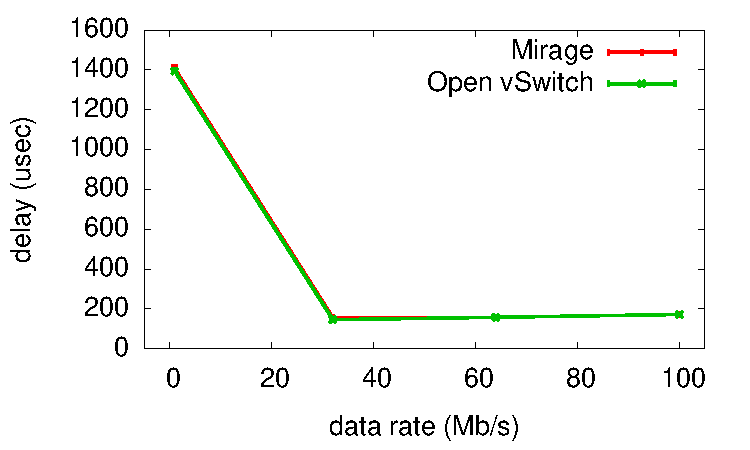
\includegraphics[width=\columnwidth]{Chapter1/Chapter1Figs/switch-media-delay}
\caption[\of switch data pane evaluation]{\label{fig:switch}Min/max/median
delay switching 100\,byte packets when running the Mirage switch and \ovs
kernel module as DomU virtual machines.}
\end{figure}

Figure~\ref{fig:switch} plots as error boxes the minimum, median and maximum of the
median processing latency of ten test runs of the experiment. We can see that
the \mirage switch's forwarding performance is very close to that of the \ovs,
even mirroring the high per-packet processing latency with a probe rate of
1 Mbps; we believe this is due to a performance artefact of the underlying Dom0
network stack. We omitted packet loss data, but can report that both implementations
suffer similar levels of packet loss.  From the comparison results of the
\mirage \of switch, we can conclude that our \of switch can emulate accurately
software switch functionality. Nonetheless, the minimum latency of our switch
emulation (approximately 100 ms) is 2 order of magnitude higher than a
hardware switch (approximately 0.5-1 $\mu$s). This performance difference can
be bridged easily using the time dilation functionality with TDF=100.

Furthermore, using the results from the evaluation of Switch4 (Section~\ref{sec:oflops-result}),
we configured our switch model to evaluate the switch modelling functionality of \sdnsim.
We set-up a simple topology with two hosts, a \textit{data sink}, and a \textit{data generation} host,
interconnected through an \of switch. The data sink host generates flow
requests to the data generation host following an exponential distribution with
$\lambda=0.02$ and a constant request size of 1MB\@. The measurement probe achieves an average
200 Mbps data rate. We ran our experiment for 120 seconds, ensuring that the
resulting number of flows is below the flow table limits. For all experiments we
used a learning switch control application.

\begin{figure}[t] 
  \centering
  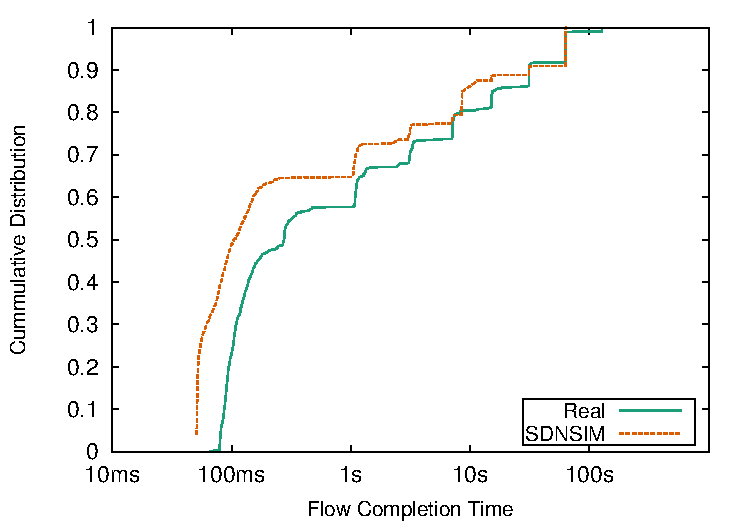
\includegraphics[width=0.70\textwidth]{Chapter1/Chapter1Figs/2hosts-cumm} 
  \caption[Flow completion time cumulative distribution using Switch4 and an
  \sdnsim emulation model]{Flow completion time cumulative distribution for a
  real setup using Switch4 and an \sdnsim emulation using a model switch. The
  switch model can approximate with high accuracy the behaviour of the
  real system.} 
  \label{fig:eval:switch-perf} 
\end{figure}


Figure~\ref{fig:eval:switch-perf} presents the cumulative distribution of flow
completion times for the real and model-based switch. The results highlight the
impact of the switch control plane design on data plane performance.  In the
real experiment, 20\% of flows have higher completions time than 10 seconds.
The predominant cause of this effect is the rate-limiting behaviour of the
switch in \texttt{pkt\_in} message transmissions. This results in TCP SYN and
SYNACK packet drops and retransmissions during ``bursty'' periods. The
completion time distribution exhibits a stepping behaviour, aligned with the
back-off delay mechanism of TCP in the SYN\_SENT/SYN\_RCVD states\footnote{In
    our experiments we are using Linux hosts with kernel 3.11.0, which
incorporates TCP Fast Open~\cite{Cheng13}.}. Our model is able to capture the
macroscopic behaviour of the switch, but exhibits a minor completion time
overestimation. We attribute this behaviour to the high load that the reactive
control scheme introduces to the communication channel between the co-processor
of the switch and the ASIC, which skews the measured behaviour at run-time.

\subsection{\ns{3} Simulation Scalability} \label{sec:sdnsim-ns3-perf}

\begin{figure}[ht]
\subfigure[centralised topology]{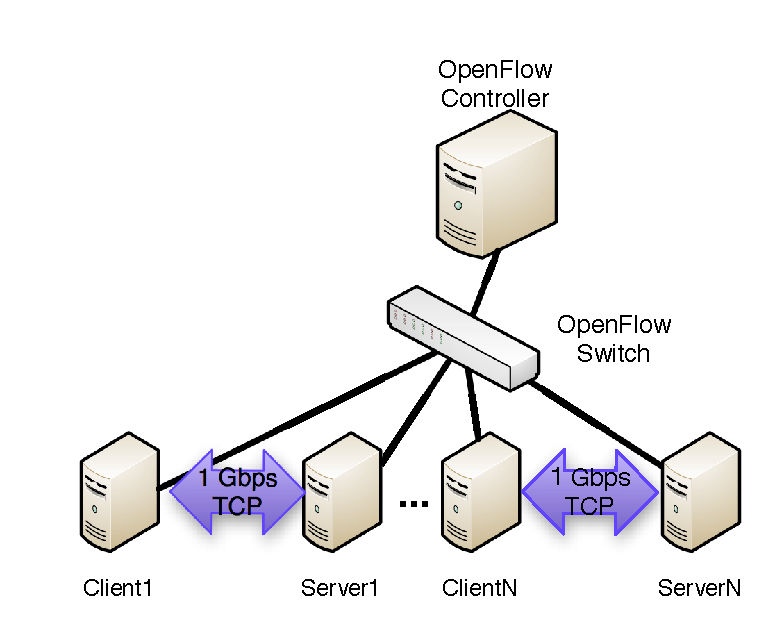
\includegraphics[width=0.45\textwidth]{Chapter1/Chapter1Figs/sdnsim-topology-single}\label{fig:sdnsim-ns3-simulation-single}}
\subfigure[distributed topology] {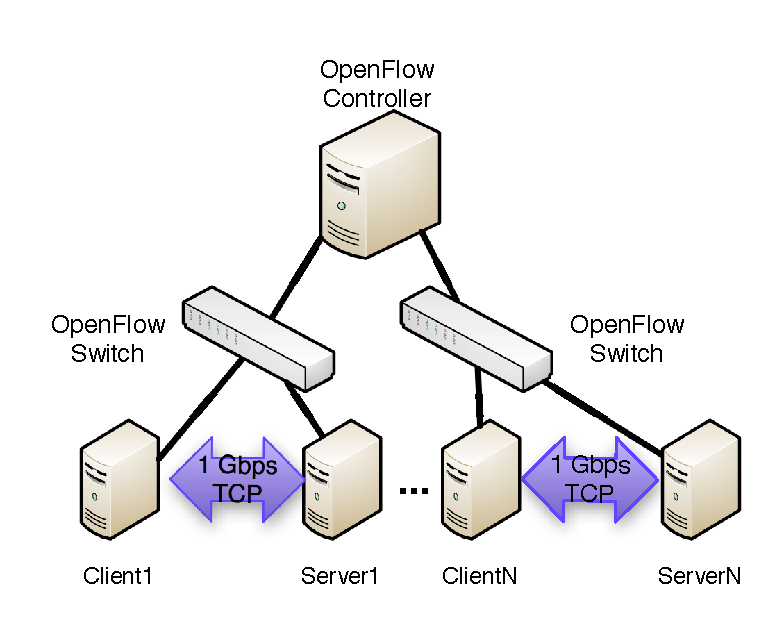
\includegraphics[width=0.45\textwidth]{Chapter1/Chapter1Figs/sdnsim-topology-double}\label{fig:sdnsim-ns3-simulation-double}}
\caption[\ns{3} scalability evaluation topology]{Network topology to test the
scalability of \ns{3}-based simulation. We simulated two topologies: a
centralised topology~(Figure~\ref{fig:sdnsim-ns3-simulation-single}) and a
distributed topology~(Figure~\ref{fig:sdnsim-ns3-simulation-double}).}
\label{fig:sdnsim-ns3-simulation}
\end{figure}

\begin{table}
\begin{center}
\begin{tabular}{|l|c|c|c|c|c|c|} \hline
&\multicolumn{3}{|c|}{Centralised topology} & \multicolumn{3}{|c|}{Distributed
  topology} \\
\cline{2-7}
Number of hosts & 4 & 8 & 12 & 4 & 8 & 12 \\
\hline 
Wall-clock delay (in min) & 13 & 35 & 75 & 8 & 25 & 42 \\
\hline
Slowdown factor & 26 & 70 & 150 & 16 & 50 & 84 \\
\hline 
\end{tabular}
\end{center}
\caption[Wall-clock delay to run 30 seconds of simulation time.]{Wall-clock
delay to run 30 seconds of simulation time of the experiment in
Figure~\ref{fig:sdnsim-ns3-simulation}, with a varying number of network hosts.
\sdnsim simulation using the \ns{3} backend scales
linearly when the traffic is localised.}
\label{tbl:sdnsim-ns3-simulation-results}
\end{table}

We evaluated the \sdnsim simulation scalability using a simple network topology,
depicted in Figure~\ref{fig:sdnsim-ns3-simulation}.  The topology consisted of a
number of switches and host pairs, connected through 1 GbE links.  Each pair of
hosts generated steady state TCP traffic at line rate.  We used two variations of
the topology: a \textit{centralised topology} \/using a single switch to connect
all hosts (Figure~\ref{fig:sdnsim-ns3-simulation-single}), and a
\textit{distributed topology}, with pairs of hosts distributed between two
switches (Figure~\ref{fig:sdnsim-ns3-simulation-double}).  Each switch is
connected to a controller running a learning switch application. 

We executed 30 seconds of simulation time on a 24-core AMD server with 128 GB of
RAM and present in Table~\ref{tbl:sdnsim-ns3-simulation-results} the wall-clock
execution time and the slowdown factor of each simulation.  From the results we
note that the real time to execute a simulation in \sdnsim depends on the number
of network events; as we increase the number of host and, consequently, the
number of packets, the execution time increases.  Additionally, from the
comparison between the centralised and distributed topology, we note that the
performance of the simulation improves when network events are localized, as the
simulation can be parallelised. In the distributed topology, network events are
distributed between the two switches and execute independently, achieving
near-linear scaling. The scaling properties of the \sdnsim simulation backend
matches datacenter traffic experimentation, where application run
independently and networks employ multipath topologies~\mycite{Kandula09}. 

\section{Hierarchical Distributed Control}\label{sec:rdsf-eval}

\begin{figure}[h]
  \begin{center}
    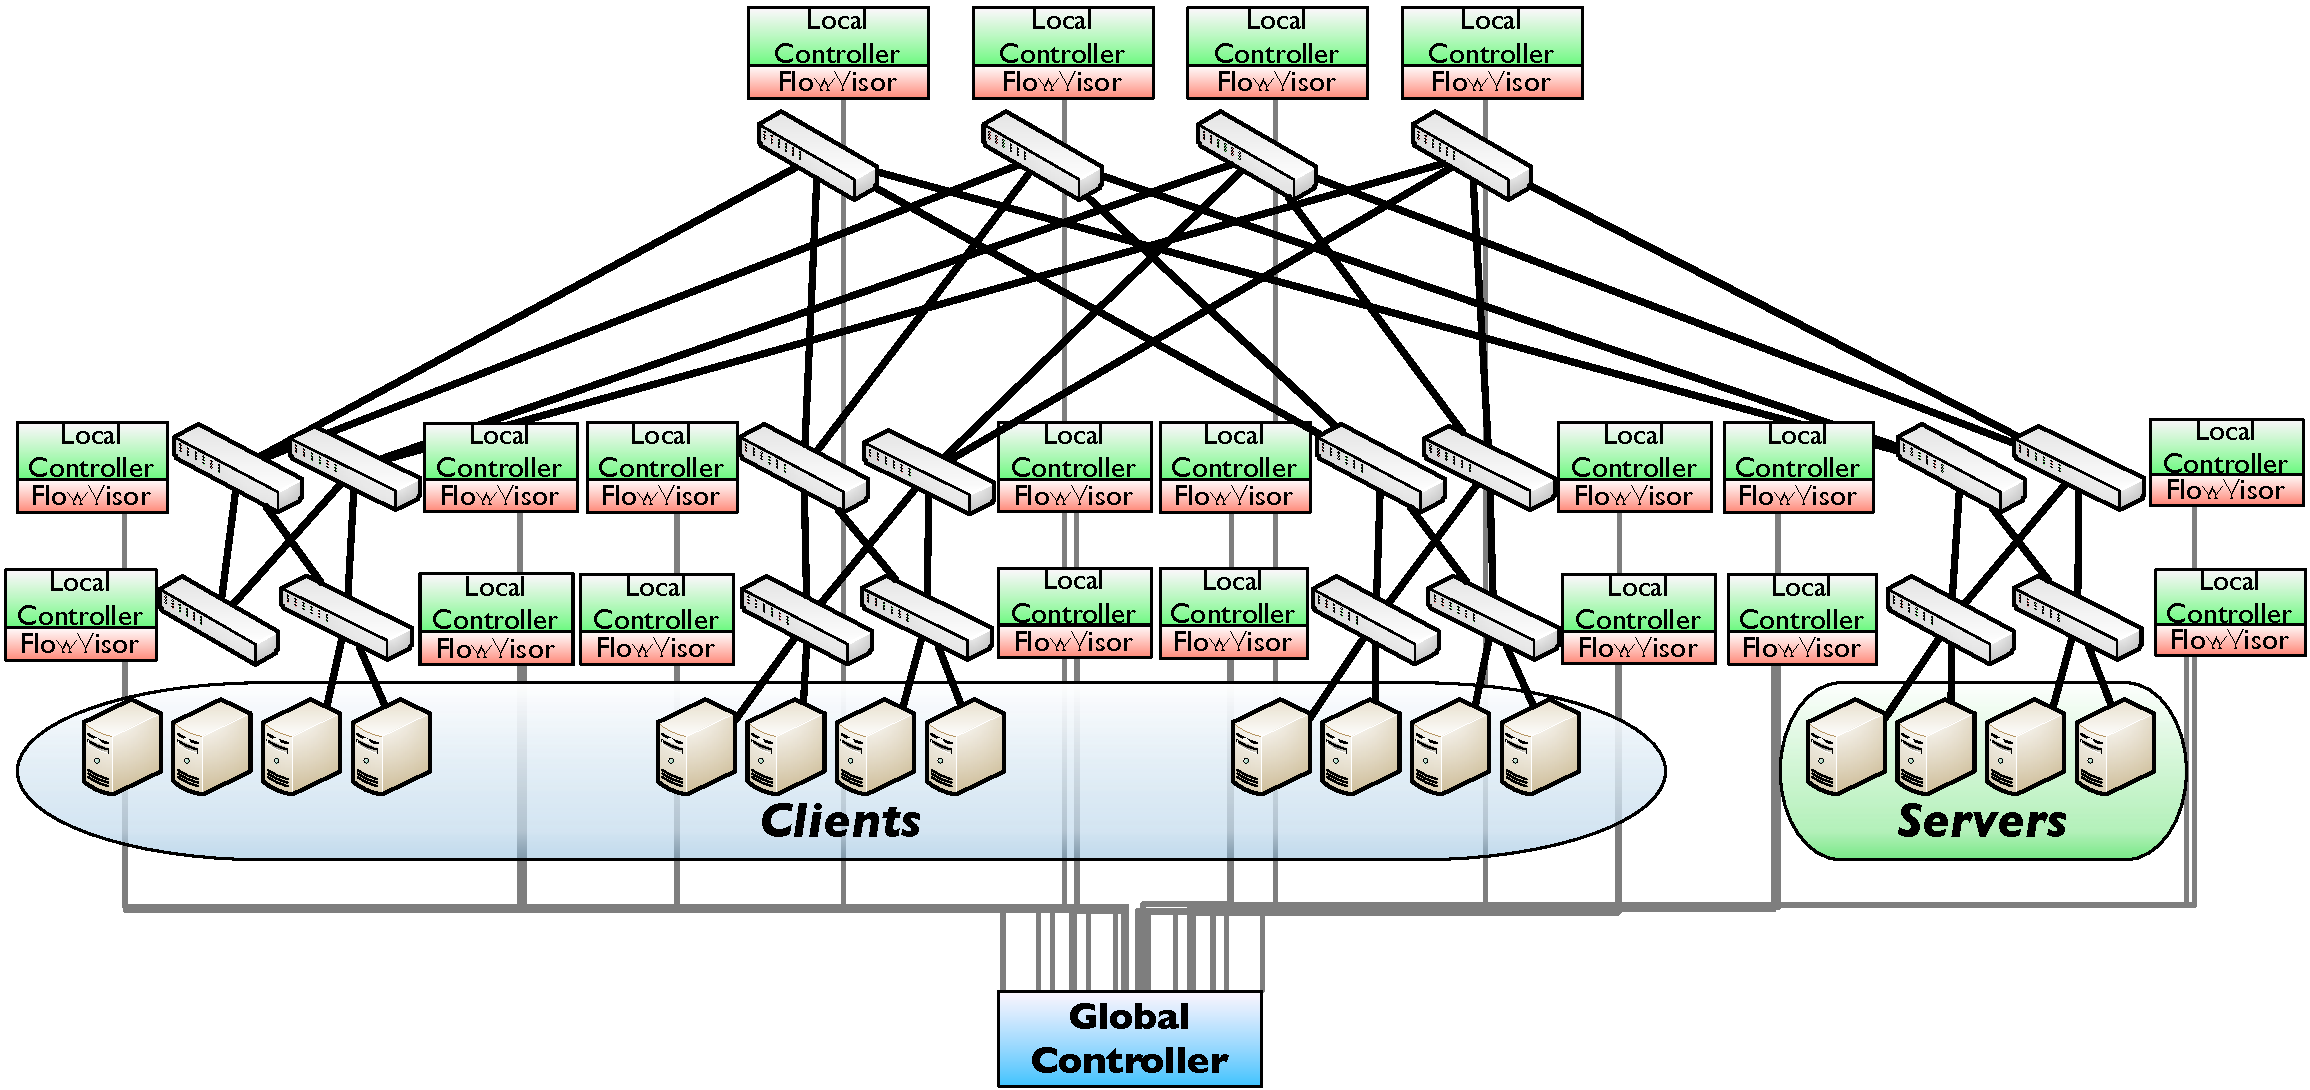
\includegraphics[width=0.99\textwidth]{Chapter1/Chapter1Figs/hierarchy-topology}
  \end{center}
  \caption{Hierarchical control experimental topology.}
  \label{fig:sdnsim-use-case-topology}
\end{figure}

As we have discussed earlier in Section~\ref{sec:background:ofapp}, the \of
abstraction can be used both for reactive and proactive control.  The two
approaches represent the two extremes of the control spectrum: proactive
control pre-computes forwarding policy and thus reduces control plane latency;
while reactive control enables unprecedented fine levels of network control at
the cost of latency and scalability.  In this section we present a use case for
\sdnsim, evaluating the impact of distributed reactive control in network
performance. 

The experimental design revisits the hierarchical design pattern on network
control distribution. Specifically, a global controller connects to all network
devices and maintains a global view of the network, while local controllers
connect to a subset of the devices and exercise local forwarding policy in
order to improve control responsiveness when necessary. A \flv instance on each
network device multiplex switch control channels between local and global
controllers, and can dynamically delegate control between the two controllers.
During periods with high control plane load, the architecture can switch
control to the local controllers in order to improve latency and reduce the
load on the central controller.  Our experimental scenario simulates this control
architecture and evaluates the impact of multi-level control on 
data plane performance.

The experiment, presented in Figure~\ref{fig:sdnsim-use-case-topology}, uses a
FatTree Clos topology with 4 pods and replicates the network behaviour of a
database application. Specifically,  the hosts in the first three pods act as
clients, while the hosts of the fourth pod act as database servers. Each client
selects uniformly at random a server  and generates a 10 byte request, which is
fulfilled by the server. The request size is selected uniformly at random from
the values of 4 KB, 8 KB, 16 KB, 32 KB and 64 KB\@, while request arrivals
follow a Poisson model. The control architecture of the network replicates the
control logic presented by~\mycitet{Al-Fares08}.  Every second the controller
polls for flow-level statistics, calculates link loads, and redistributes flows
between redundant network paths. In addition, the controller distributes new
flow between redundant paths, with probabilities proportional to the path load
ratio. The experiment tries to recreate with high fidelity the impact of SDN
control in network functionality. In order to achieve this, we use a switch
model based on  the performance characteristics of Switch4. Nonetheless, the
measured performance characteristics of Switch4 cannot accommodate the flow
arrival rate exhibited by the employed traffic model. For example, the switch
requires approximately 1 ms to install a flow in the flow table and the
employed arrival rate of 250 flows per second would create a queue with
utilization $\rho>1$. As a result, we improve the performance of the employed
model by an order of magnitude in order to support the experimental event
rates. Our experimental definition incorporates additional experimental
parameter regarding the controller performance characteristics and processing
and propagation delays, presented in
Table~\ref{tbl:sdnsim_experiment_parameters}.

\begin{table}
\begin{center}
\begin{tabular}{|c| l |} \hline
  Parameter & value \\ \hline
  packet\_in processing delay & 10 $\mu$sec \\ \hline
  flow\_mod insertion delay & 120 $\mu$sec \\ \hline
  link propagation delay & 0.5 $\mu$sec \\ \hline
  switch processing delay & 10 $\mu$sec \\ \hline
  link capacity & 100 Mbps \\ \hline
  Request arrival rate (per host) & 62 retrievals/sec \\ \hline
  Network device queue size & 100 packets \\ \hline
\end{tabular}
\end{center}
\label{tbl:sdnsim_experiment_parameters}
\caption{Hierarchical control simulation parameters.}
\end{table}

Using the previous experimental setup, we evaluated the impact of distributed
and centralised control. Distributed control uses only local controllers and
defines the forwarding policy using the traffic matrix of a single switch. In
this setup we assume that a local controller has minimum latency to access
the switch and minimizes the control channel latency and load. Global control
uses only the global controller and setups end-to-end paths on a per-flow basis
using the network-wide traffic matrix.

We evaluate the effect of each control scheme on data plane performance using
the flow completion time metric, as proposed by relevant
research~\mycite{Dukkipati2006}. Figure~\ref{fig:sdnsim-use-case-result}
presents the median, 10$^{th}$ and 90$^{th}$ quantiles of the completion time
distribution for each flow size and for each control scheme. From the results
we note two important observation. Firstly, the results point out the
significant non-linear increase in flow completion time between short (4 KB and
8 KB) and long flows (16 KB, 32 KB and 64 KB). This result is a direct
consequence of the TCP slow start behaviour, as discussed
by~\citet{Dukkipati10}. Mirage uses an initial TCP window size of 5840 bytes,
sufficient to transmit all flow bytes within the slow start phase for short
flows. Longer flows increase their window slower and thus increase the
probability to experience transient queueing latencies. Secondly, the
centralised policy improves resource utilisation across the network and thus
reduces the effect of network queueing delays. Although the distributed
approach exhibits lower control channel propagation delay, the suboptimal
forwarding policy of the system increase the flow completion time, especially
for long-lived TCP connections. More specifically, distributed control
increases the median completion time by 2 ms in comparison to centralised
control, while for 4 KB flows the delay increase is limited to 200 $\mu$s.
Distributed control can reduce the impact of control channel latency during
high flow arrival rates, incurs a significant non-negligible data plane
performance degradation.



\begin{figure}[h]
  \begin{center}
    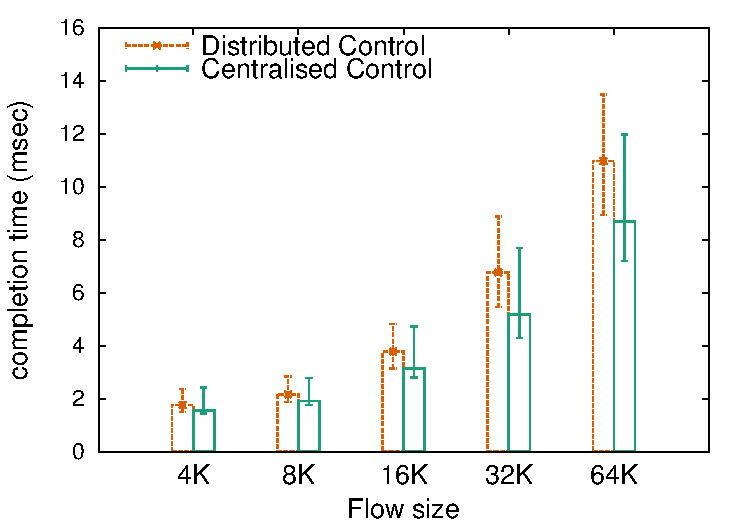
\includegraphics[width=0.80\textwidth]{Chapter1/Chapter1Figs/sdnsim-use-case}
  \end{center}
  \caption[Hierarchical control evaluation using TCP flow completion
  time]{Comparison of TCP flow completion time for various flow sizes between a
  centralised and decentralised control architecture on a Fat-Tree topology.}
  \label{fig:sdnsim-use-case-result}
\end{figure}


\section{Summary} \label{sec:modeling:summary}

This chapter discussed the scalability of the predominant SDN
implementation, the \of protocol.  We presented \oflops, a tool that tests the
capabilities and performance of \of-enabled software and hardware switches.
\oflops combines advanced hardware instrumentation, for accuracy and
performance, and provides an extensible software framework. We used \oflops to
evaluate six different \of switch implementations, in terms of \of
protocol support as well as performance.  In our performance evaluation, we
benchmarked the packet processing, traffic interception and injection, flow table
modification and traffic statistics export functionalities of the switches.  We
identified considerable variation among the tested \of implementations.  We took
advantage of the ability of \oflops for data plane measurements to quantify
accurately how fast switches process and apply \of commands.  For example, we
found that the \texttt{barrier} reply message is not correctly implemented,
making it difficult to predict when flow operations will be seen by the data
plane.  Finally, we found that the monitoring capabilities of existing hardware
switches have limitations in their ability to sustain high rates of requests.
Furthermore, at high rates, monitoring operations impact other \of commands.

In addition, in this chapter we presented the \sdnsim platform, an experimentation
framework for large-scale high-precision experimentation with control plane
architectures. \sdnsim used the \mirage abstraction and application libraries to enable
experimenters to program the functionality of their network. An \sdnsim experiment
definition can seamlessly translate at compile time into a simulation over the \ns{3}
simulation platform, or a high precision emulation over the Xen virtualisation
framework. We conducted a number of micro-benchmarks and evaluated that the
software provided emulation performance comparable to software \of controller and
switching platforms, while \sdnsim simulation provided good scaling properties.
Furthermore, we used \sdnsim to investigate the impact of hierarchical distributed
control architectures on the performance of the data plane of the network.  In
the next chapter, we explore applications of the SDN paradigm to scale network
management. 

